% XeLaTeX can use any Mac OS X font. See the setromanfont command below.
% Input to XeLaTeX is full Unicode, so Unicode characters can be typed directly into the source.

% The next lines tell TeXShop to typeset with xelatex, and to open and save the source with Unicode encoding.

%!TEX TS-program = xelatex
%!TEX encoding = UTF-8 Unicode

\documentclass[a4paper,bachelor]{ructhesis}

%自添宏包
\usepackage{skak}%国际象棋
\usepackage{subfigure}%子图http://www.ctex.org/documents/latex/graphics/node111.html
\usepackage{chemfig}%化学式
\usepackage{extarrows}%长等号
%\usepackage{subfig}%并列图片
\usetikzlibrary{trees}

\usepackage{color}
\usepackage{fancyvrb}
\usepackage[bottom]{footmisc}
\newcommand{\VerbBar}{|}
\newcommand{\VERB}{\Verb[commandchars=\\\{\}]}
\DefineVerbatimEnvironment{Highlighting}{Verbatim}{commandchars=\\\{\}}
% Add ',fontsize=\small' for more characters per line
\usepackage{framed}
\definecolor{shadecolor}{RGB}{248,248,248}
\newenvironment{Shaded}{\begin{snugshade}}{\end{snugshade}}
\newcommand{\KeywordTok}[1]{\textcolor[rgb]{0.13,0.29,0.53}{\textbf{#1}}}
\newcommand{\DataTypeTok}[1]{\textcolor[rgb]{0.13,0.29,0.53}{#1}}
\newcommand{\DecValTok}[1]{\textcolor[rgb]{0.00,0.00,0.81}{#1}}
\newcommand{\BaseNTok}[1]{\textcolor[rgb]{0.00,0.00,0.81}{#1}}
\newcommand{\FloatTok}[1]{\textcolor[rgb]{0.00,0.00,0.81}{#1}}
\newcommand{\ConstantTok}[1]{\textcolor[rgb]{0.00,0.00,0.00}{#1}}
\newcommand{\CharTok}[1]{\textcolor[rgb]{0.31,0.60,0.02}{#1}}
\newcommand{\SpecialCharTok}[1]{\textcolor[rgb]{0.00,0.00,0.00}{#1}}
\newcommand{\StringTok}[1]{\textcolor[rgb]{0.31,0.60,0.02}{#1}}
\newcommand{\VerbatimStringTok}[1]{\textcolor[rgb]{0.31,0.60,0.02}{#1}}
\newcommand{\SpecialStringTok}[1]{\textcolor[rgb]{0.31,0.60,0.02}{#1}}
\newcommand{\ImportTok}[1]{#1}
\newcommand{\CommentTok}[1]{\textcolor[rgb]{0.56,0.35,0.01}{\textit{#1}}}
\newcommand{\DocumentationTok}[1]{\textcolor[rgb]{0.56,0.35,0.01}{\textbf{\textit{#1}}}}
\newcommand{\AnnotationTok}[1]{\textcolor[rgb]{0.56,0.35,0.01}{\textbf{\textit{#1}}}}
\newcommand{\CommentVarTok}[1]{\textcolor[rgb]{0.56,0.35,0.01}{\textbf{\textit{#1}}}}
\newcommand{\OtherTok}[1]{\textcolor[rgb]{0.56,0.35,0.01}{#1}}
\newcommand{\FunctionTok}[1]{\textcolor[rgb]{0.00,0.00,0.00}{#1}}
\newcommand{\VariableTok}[1]{\textcolor[rgb]{0.00,0.00,0.00}{#1}}
\newcommand{\ControlFlowTok}[1]{\textcolor[rgb]{0.13,0.29,0.53}{\textbf{#1}}}
\newcommand{\OperatorTok}[1]{\textcolor[rgb]{0.81,0.36,0.00}{\textbf{#1}}}
\newcommand{\BuiltInTok}[1]{#1}
\newcommand{\ExtensionTok}[1]{#1}
\newcommand{\PreprocessorTok}[1]{\textcolor[rgb]{0.56,0.35,0.01}{\textit{#1}}}
\newcommand{\AttributeTok}[1]{\textcolor[rgb]{0.77,0.63,0.00}{#1}}
\newcommand{\RegionMarkerTok}[1]{#1}
\newcommand{\InformationTok}[1]{\textcolor[rgb]{0.56,0.35,0.01}{\textbf{\textit{#1}}}}
\newcommand{\WarningTok}[1]{\textcolor[rgb]{0.56,0.35,0.01}{\textbf{\textit{#1}}}}
\newcommand{\AlertTok}[1]{\textcolor[rgb]{0.94,0.16,0.16}{#1}}
\newcommand{\ErrorTok}[1]{\textcolor[rgb]{0.64,0.00,0.00}{\textbf{#1}}}
\newcommand{\NormalTok}[1]{#1}

%将封面信息补全

%文头
  \sign{中国人民大学本科毕业论文} 




% 以下信息本科研究生都需要补全
\title{论贸易战对中国未来经济的影响} %论文题名,论文的正标题
\author{yimeng} %论文作者姓名
\school{统计学院} %论文作者所在学院的全称
\field{经济统计学} %论文作者所学专业的全称;相关专业名称过长的请在文字前添加命令\ziju{-0.15}
\studentid{20163160102} %论文作者的学号
\advisor{yalei} %指导老师的亲笔签名
\date{2018-09-30} %论文小组评阅或答辩日期


% 以下本科填写
\grade{} %论文作者所在年级,如:2014级。
\score{4.0} %由学院毕业论文评审小组或学院毕业论文答辩委员会最终确认的毕业论文成绩
\thesiscode{论文编码:RUC-BK-专业代码-学号 RUC-BK-050101-2014201237} %论文编码由学校代码、类别代码、专业代码、学号组成,专业代码详见教务处网站文件下载区。例如:RUC-BK-050101-2014201237。
\subtitle{基于统计模拟的经济学预测方法} %本项目为任选项目,指论文的副标题,即对论文题名的解释或补充说明


%以下研究生填写 本科生不需要填写

%摘要关键词:本科研究生都需要填写!
\keywordzh{
贸易战 \qquad
经济 \qquad
} %中文摘要关键词,词间间隔3格,用{ }{ }{ }实现,方法不唯一


\keyworden{
Trade War \qquad
Economics \qquad
} %外文摘要关键词,互相之间间隔3格


%
\usepackage{amsthm}
\newtheorem{theorem}{Theorem}[chapter]
\newtheorem{lemma}{Lemma}[chapter]
\theoremstyle{definition}
\newtheorem{definition}{Definition}[chapter]
\newtheorem{corollary}{Corollary}[chapter]
\newtheorem{proposition}{Proposition}[chapter]
\theoremstyle{definition}
\newtheorem{example}{Example}[chapter]
\theoremstyle{definition}
\newtheorem{exercise}{Exercise}[chapter]
\theoremstyle{remark}
\newtheorem*{remark}{Remark}
\newtheorem*{solution}{Solution}
\begin{document}

%扉页
\maketitle


%中文摘要
% \begin{abstractzh}
    RUCThesis 是根据中国人民大学《本科论文指导手册》和《研究生学位论文及其摘要的撰写和印制要求》而制作的 \LaTeX\ 论文模板。
\end{abstractzh}
\begin{abstractzh}
  中文摘要: RUCThesis
  是根据中国人民大学《本科论文指导手册》和《研究生学位论文及其摘要的撰写和印制要求》而制作的
  \LaTeX~论文模板。
\end{abstractzh}

%英文摘要
% % the abstract
\begin{abstracten}
    This is an English Abstract.
\end{abstracten}
\begin{abstracten}
  This is a English abstract.
\end{abstracten}


\frontmatter

%正文目录
\tableofcontents
%插图目录
\listoffigures
%表格目录
\listoftables


\mainmatter\clearpage
\pagestyle{fancy}

%正文章节
\hypertarget{bookdown}{%
\chapter{bookdown介绍}\label{bookdown}}

This is a \emph{sample} book written in \textbf{Markdown}. You can use
anything that Pandoc's Markdown supports, e.g., a math equation
\(a^2 + b^2 = c^2\).

The \textbf{bookdown} package can be installed from CRAN or Github:

\begin{Shaded}
\begin{Highlighting}[]
\KeywordTok{install.packages}\NormalTok{(}\StringTok{"bookdown"}\NormalTok{)}
\CommentTok{# or the development version}
\CommentTok{# devtools::install_github("rstudio/bookdown")}
\end{Highlighting}
\end{Shaded}

Remember each Rmd file contains one and only one chapter, and a chapter
is defined by the first-level heading \texttt{\#}.

每一个Rmd文件只包含一章内容,每一章由一个一级标题\texttt{\#}来指定。

To compile this example to PDF, you need XeLaTeX. You are recommended to
install TinyTeX (which includes XeLaTeX):
\url{https://yihui.name/tinytex/}.

你需要安装XeLaTeX来将这个示例编译为PDF,推荐你去
\href{https://yihui.name/tinytex/}{这个网站}
安装TinyTex,它是包含XeLaTex的。

\hypertarget{intro}{%
\chapter{引言}\label{intro}}

You can label chapter and section titles using \texttt{\{\#label\}}
after them, e.g., we can reference Chapter \ref{intro}. If you do not
manually label them, there will be automatic labels anyway, e.g.,
Chapter \ref{methods}.

Figures and tables with captions will be placed in \texttt{figure} and
\texttt{table} environments, respectively.

\begin{Shaded}
\begin{Highlighting}[]
\KeywordTok{par}\NormalTok{(}\DataTypeTok{mar =} \KeywordTok{c}\NormalTok{(}\DecValTok{4}\NormalTok{, }\DecValTok{4}\NormalTok{, }\FloatTok{.1}\NormalTok{, }\FloatTok{.1}\NormalTok{))}
\KeywordTok{plot}\NormalTok{(pressure, }\DataTypeTok{type =} \StringTok{'b'}\NormalTok{, }\DataTypeTok{pch =} \DecValTok{19}\NormalTok{)}
\end{Highlighting}
\end{Shaded}

\begin{figure}

{\centering 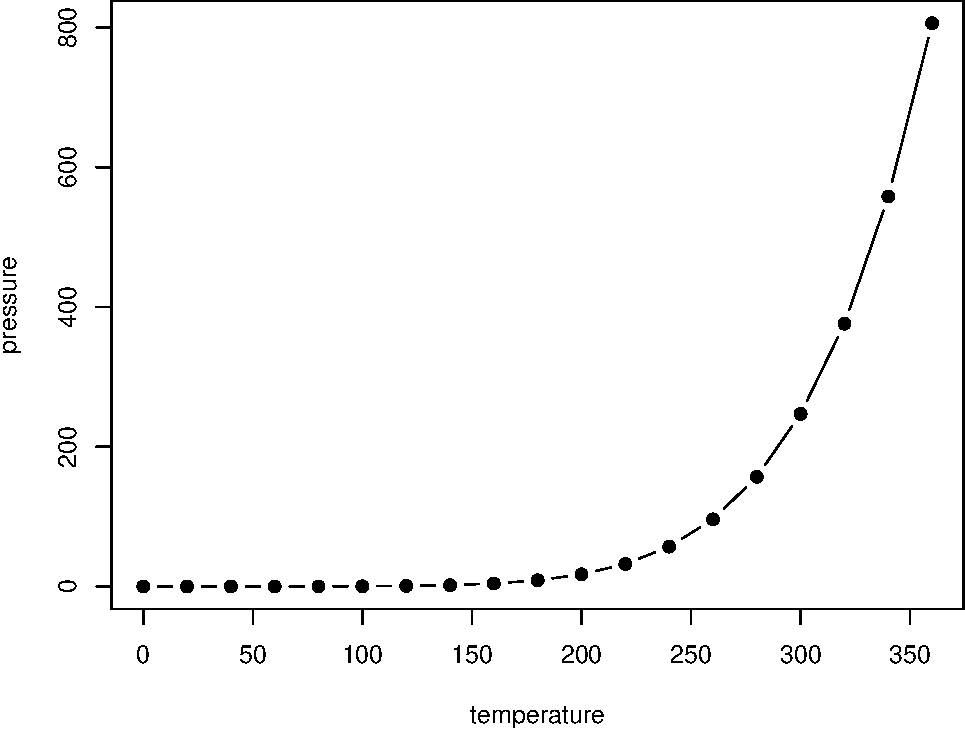
\includegraphics[width=0.8\linewidth]{RUC_files/figure-latex/nice-fig-1} 

}

\caption{气温和气压关系图}\label{fig:nice-fig}
\end{figure}

Reference a figure by its code chunk label with the \texttt{fig:}
prefix, e.g., see Figure \ref{fig:nice-fig}. Similarly, you can
reference tables generated from \texttt{knitr::kable()}, e.g., see Table
\ref{tab:nice-tab}.

\begin{Shaded}
\begin{Highlighting}[]
\NormalTok{knitr}\OperatorTok{::}\KeywordTok{kable}\NormalTok{(}
  \KeywordTok{head}\NormalTok{(iris, }\DecValTok{20}\NormalTok{), }\DataTypeTok{caption =} \StringTok{'示例表格'}\NormalTok{,}
  \DataTypeTok{booktabs =} \OtherTok{TRUE}
\NormalTok{)}
\end{Highlighting}
\end{Shaded}

\begin{table}

\caption{\label{tab:nice-tab}示例表格}
\centering
\begin{tabular}[t]{rrrrl}
\toprule
Sepal.Length & Sepal.Width & Petal.Length & Petal.Width & Species\\
\midrule
5.1 & 3.5 & 1.4 & 0.2 & setosa\\
4.9 & 3.0 & 1.4 & 0.2 & setosa\\
4.7 & 3.2 & 1.3 & 0.2 & setosa\\
4.6 & 3.1 & 1.5 & 0.2 & setosa\\
5.0 & 3.6 & 1.4 & 0.2 & setosa\\
\addlinespace
5.4 & 3.9 & 1.7 & 0.4 & setosa\\
4.6 & 3.4 & 1.4 & 0.3 & setosa\\
5.0 & 3.4 & 1.5 & 0.2 & setosa\\
4.4 & 2.9 & 1.4 & 0.2 & setosa\\
4.9 & 3.1 & 1.5 & 0.1 & setosa\\
\addlinespace
5.4 & 3.7 & 1.5 & 0.2 & setosa\\
4.8 & 3.4 & 1.6 & 0.2 & setosa\\
4.8 & 3.0 & 1.4 & 0.1 & setosa\\
4.3 & 3.0 & 1.1 & 0.1 & setosa\\
5.8 & 4.0 & 1.2 & 0.2 & setosa\\
\addlinespace
5.7 & 4.4 & 1.5 & 0.4 & setosa\\
5.4 & 3.9 & 1.3 & 0.4 & setosa\\
5.1 & 3.5 & 1.4 & 0.3 & setosa\\
5.7 & 3.8 & 1.7 & 0.3 & setosa\\
5.1 & 3.8 & 1.5 & 0.3 & setosa\\
\bottomrule
\end{tabular}
\end{table}

You can write citations, too. For example, we are using the
\textbf{bookdown} package \citep{R-bookdown} in this sample book, which
was built on top of R Markdown and \textbf{knitr} \citep{xie2015}.

\chapter{文献综述}

Here is a review of existing methods.

这个示例我们使用了\textbf{bookdown}包\citep{R-bookdown},它是建立在R
Markdown和\textbf{knitr}\citep{xie2015}基础上的。

\chapter{研究方法}

插入一个pdf文件(图片文件),使得其宽度为页面左右边距:

\begin{Shaded}
\begin{Highlighting}[]
\NormalTok{knitr}\OperatorTok{::}\KeywordTok{include_graphics}\NormalTok{(}\StringTok{'figures/logo.pdf'}\NormalTok{, }\DataTypeTok{auto_pdf=}\OtherTok{TRUE}\NormalTok{)}
\end{Highlighting}
\end{Shaded}

\begin{figure}

\includegraphics[width=1\linewidth]{figures/logo} \caption{中英文校徽}\label{fig:unnamed-chunk-3}
\end{figure}

We describe our methods in this chapter.

\chapter{一些应用例子}

Some \emph{significant} applications are demonstrated in this chapter.

\section{应用一:并列图片\&表格设置}

插入并列的图片:

\begin{figure}

\begin{minipage}[t]{0.5\textwidth}
  \centering
  
\includegraphics[width=0.8\textwidth]{figures/logo}
  \caption{我是左边的图}
\end{minipage}
\begin{minipage}[t]{0.5\textwidth}
  \centering
  
\includegraphics[width=0.8\textwidth]{figures/logo}
  \caption{我是右边的图}
\end{minipage}

\end{figure}

插入并列的表格:

\begin{table}
\begin{minipage}{0.5\textwidth}
  \centering
  \caption{\label{tab:t2}左边的 table}
  \begin{tabular}{c|c|c}
    \hline
    A & B & C \\
    \hline
    1 & 2 & 3  \\
    \hline
    4 & 5 & 6 \\
    \hline
  \end{tabular}
\end{minipage}
\begin{minipage}{0.5\textwidth}
  \centering
  \caption{\label{tab:t2}右边的 table}
  \begin{tabular}{c|c|c}
    \hline
    A & B & C \\
    \hline
    1 & 2 & 3  \\
    \hline
    4 & 5 & 6 \\
    \hline
  \end{tabular}
\end{minipage}
\end{table}

是的,这个图和表好像会乱跑,但是有caption就可以直接通过图表目录的链接来查看。

\section{应用二:数学环境}

插入\footnote{添加一个解释说明的脚注}数学公式:

\[
\begin{aligned}
P\{S_n \leq t\}
&= \int_{-\infty}^{+\infty}f_{S_n}dt \notag \\
&= \int_0^t\frac{\lambda(\lambda u)^{n-1}}{(n-1)!}e^{-\lambda u}du \\
&\xlongequal{\lambda u=x} \frac{1}{(n-1)!}\int_0^{\lambda t}x^{n-1}e^{-x}dx\\
&=\frac{-1}{(n-1)!}(e^{-x}x^{n-1}{\Big|}_0^{\lambda t}-\int_0^{\lambda t}e^{-x}dx^{n-1})\\
&=\frac{-1}{(n-1)!}e^{-x}x^{n-1}{\Big|}_0^{\lambda t}+\frac{1}{(n-2)!}\int_0^{\lambda t}e^{-x}x^{n-2}dx
\end{aligned}
\]

可以再插入一个数学公式\footnote{第二个脚注}:

\[    
\begin{aligned}
\lambda 
&=\left (1+\frac{\left(\frac{\bar{X}-\bar{Y}}{\sqrt{((\frac{1}{n}+\frac{1}{m})\sigma^2)}}\right)^2}{\left(\sqrt{\frac{\sum\limits_{i=1}^n(X_i-\bar{X})^2+\sum\limits_{i=1}^m(Y_i-\bar{Y})^2}{(m+n)\sigma^2}}\right)^2(m+n-2)}\right)^{\frac{n+m}{2}} \\ \notag
&=\left(1+\frac{T^2}{n+m-2}\right)^{\frac{n+m}{2}}
\end{aligned}
\]

其中,

\[
\begin{aligned}
\quad T^2 
&=\left(\frac{\frac{\bar{X}-\bar{Y}}{\sqrt{((\frac{1}{n}+\frac{1}{m})\sigma^2)}}}{{\sqrt{\frac{\sum\limits_{i=1}^n(X_i-\bar{X})^2+\sum\limits_{i=1}^m(Y_i-\bar{Y})^2}{(m+n)\sigma^2}}}}\right)^2
\end{aligned}
\]

\chapter{总结}

写完啦!

\newpage

%本科签名
\autograph


%参考文献
\bibliographystyle{ref/rucbib}
\setcitestyle{super,square,comma,sort&compress}
\bibliography{book.bib,packages.bib}
\nocite{*}
\addcontentsline{toc}{chapter}{参考文献}

%附录
\appendix
\chapter{如何正确安装\LaTeX\ }

Noun–verb dependencies in various languages and their biological ana- logues. Part A) shows the sentence “Dick saw Jane help Mary draw pictures” trans- lated grammatically into German and Dutch. That is, the words in the sentence are rearranged to reflect the rules of grammar in these two languages, but the sentence is not translated per se. As shown, the English version of the sentence has a rela- tively simple dependency structure between the nouns and verbs that can be modeled using regular grammars. In contrast, German and Dutch require more complicated grammatical models . Part B) shows the biological analogue of the three sen- tences in Part A). Typically, restriction sites can be modeled using regular grammars, whereas complex DNA secondary structures require context–free or context–sensitive grammars . In the first example, the arches are used to represent a “must be followed by” dependency. In the second two examples, they represent a “must be complementary to” dependency.


%致谢
\begin{acknowledge}%致谢
    感谢
\end{acknowledge}



\end{document}
